\section{Results and Discussion}
% mention the usage of python and implementation. % add three sigma rule here.
The three algorithms and visualizations presented in this paper are 
implemented in Python. All codes and results are available on GitHub 
(https://github.com/YupingLu/arm-pearson and https://github.com/YupingLu/arm-ssa). 
Multiple methods are available to set a threshold for extreme values as 
outliers. We used the three sigma rule to extract outliers \cite{pukelsheim1994three}. 
For example, if the distance of one point is larger than three sigmas, 
we treat this point as an outlier in Algorithm~\ref{alg:kmeans}.

% methods drawbacks and advantages
Pearson correlation coefficient is a pairwise comparison method which 
is used to detect abnormality of correlation between two variables. 
However if the two variables suddenly change in the same direction, 
their correlation may still be normal similar to their ``supposed" 
value. It is the same case if only a few points are outliers as the
correlation is determined by the majority of data points. 
As we performed the Pearson correlation 
coefficient on the seasonal level, it is not possible to track down 
to the exact day. SSA is a univariate method to detect outliers for 
each variable in the ARM data. It can quickly catch those high peak 
and drop points. But it requires the time series data to be continuous 
with no missing values. K-means is a commonly used multivariate method 
for clustering. Here we used it for outlier detection. The drawback of this method is 
that the detected outliers could be just one type of variable or 
multiple types of variable. It is hard to tell which is the case. 
As we also averaged the raw 
minute level data into day level data, some outliers may be averaged 
out by this process.

% all together as a template
One outlier may only be detected by SSA or Pearson correlation coefficient 
or K-means. Thus we combined all the three methods together as a 
whole framework. SSA and K-means are used to detect outliers whereas Pearson 
correlation coefficient can be used to detect the variables causing the anomaly 
in the K-means results by using the pairwise correlations. Figure~\ref{fig:combined} was the result of 
detected outliers for \textit{temp\_mean} from E33. The red squares 
stand for the common outliers detected by both K-means and SSA. The 
orange diamonds are the ones detected by K-means excluding the common 
outliers. And the black stars represents the outliers detected by SSA 
excluding the common outliers. We can see from the figure that more 
outliers have been detected compared to Figure~\ref{fig:ssa} and Figure~\ref{fig:kmeans}. 
Thus we applied this framework on all the test data. Table~\ref{tab:comp} 
shows the number of detected outliers. The size of common detected 
outliers is 378 by this framework.

\begin{figure*}[ht]
    \centering
    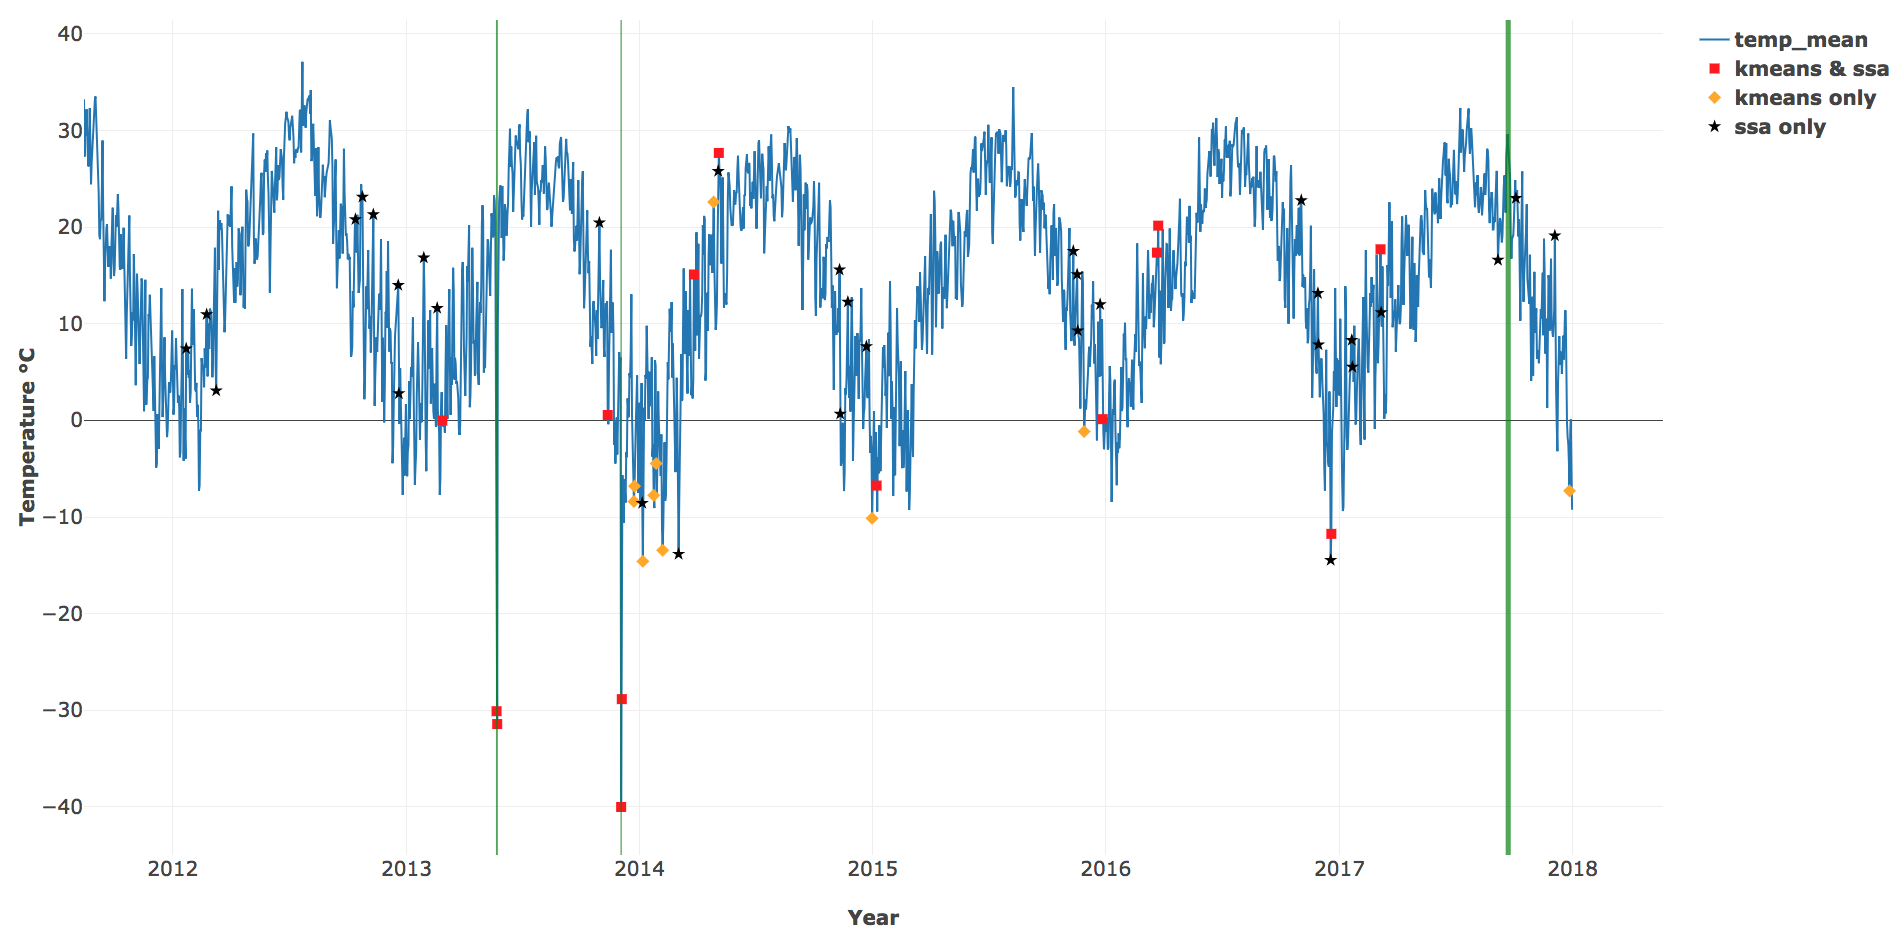
\includegraphics[width=\textwidth]{figures/combined.png}
    \caption{Outliers detected for E33 \textit{temp\_mean} using combined algorithms}
    \label{fig:combined}
\end{figure*}

\begin{table}[ht]
\caption{Comparison of SSA and K-means Outlier Set Size}
\label{tab:comp}
\centering
\begin{tabular}{|l|c|}
\cline{2-2}
\multicolumn{1}{l|}{} & Outlier Set Size\\
\hline
SSA & 922\\
K-means & 508\\
Intersection & 378\\
Symmetric Difference & 674\\
\hline
\end{tabular}
\end{table}

\begin{table}[ht]
\caption{Precision and Recall of SSA and K-means}
\label{tab:pr}
\centering
\begin{tabular}{|l|c|c|c|}
\hline
Method & Variable & Precision & Recall\\
\hline
SSA & temp\_mean & 16.00\% & 1.20\%\\
SSA & vapor\_pressure\_mean & 20.70\% & 1.40\%\\
SSA & atmos\_pressure & 0.00\% & 0.00\%\\
SSA & rh\_mean & 14.80\% & 0.50\%\\
SSA & wspd\_arith\_mean & 0.60\% & 1.50\%\\
Kmeans & 5 together & 12.90\% & 1.90\%\\
Combined & 5 together & 11.10\% & 4.10\%\\
\hline
\end{tabular}
\end{table}

% DQR here
The current data quality or outlier detection is maintained as data 
quality reports (DQRs) stored in the DQR database with each entered 
manually \cite{mccord2016arm}. A description of an event which 
changed the normal data is included in these DQRs. The event could 
be temporary operating conditions such as power failures, frozen 
and snow covered sensors, instrument degradation, or contamination. 
It could also be an extreme weather event that has never been observed 
before. Each DQR entry also contains a specific time range affected, 
list of data projects, and specific measurements. And these entries 
are usually submitted by either the Data Quality Office \cite{peppler2016arm} 
or the instrument mentor \cite{cress2016deploying}. It is easy to 
notice that this method is not efficient as it requires a lot of labor. 
It is also nearly impossible to detect all the outliers due to the 
complexity and high volume of the ARM data.

Currently, not many outliers entries are stored in DQR database. Here we 
used manually detected 181 outliers in the DQR database as the ground 
truth to compare with the results from our framework. Precision and 
recall which were first defined in \cite{perry1955machine} were used 
as the comparison metric. They are commonly used to measure the quality 
of classification tasks \cite{olson2008advanced}. Precision is calculated 
as True Positives divided by the sum of True Positives and False 
Positives. On the other hand, recall is measured from True Positives 
divided by the sum of True Positives and False Negatives. We treated 
outliers in DQR database as True Positives. Thus detected outliers not 
in the DQR database are False Positives. Undetected values which in 
the DQR database are False Negatives, and which not in the DQR database 
are True Negatives. Table~\ref{tab:pr} contains the statistics of 
the comparison.

Precision attempts to answer the proportion of positive identifications that
was actually correct. The Combined precision is 11.10\% which shows that 
many outliers detected by the framework are not in the DQR database. 
Recall tries to solve the proportion of actual positives identified 
correctly. The number is 4.10\% which is even smaller than precision. 
One reason for small recall is that the size of True Positives 
is much small. The other reason is that DQR database records the whole 
possible affected time range which makes the size of False Negatives 
large. It could be possible that only a few days of the data recorded 
during that time range are actually outliers.

